% flashcards-title: A whole split into a known and an unknown part
% flashcards-desc: A horizontal bar labeled total nine is split into a part labeled five and a hatched unlabeled part.
\documentclass[dvisvgm,tikz,border=8pt]{standalone}
\usetikzlibrary{arrows.meta,patterns}

\definecolor{qraNavy}{HTML}{17324D}
\definecolor{qraBlue}{HTML}{2B6CB0}
\definecolor{qraGold}{HTML}{B7791F}
\definecolor{qraPale}{HTML}{EAF2F8}
\definecolor{qraGray}{HTML}{5C6773}

\tikzset{
  qra axis/.style={draw=qraNavy, line width=1.2pt},
  qra tick/.style={draw=qraNavy, line width=1pt},
  qra guide/.style={draw=qraGray, densely dashed, line width=0.8pt},
  qra counter/.style={circle, draw=qraNavy, fill=qraPale, line width=0.9pt, minimum size=7mm, inner sep=0pt},
  qra label/.style={font=\sffamily\bfseries, text=qraNavy},
  qra small label/.style={font=\sffamily, text=qraNavy},
}

\begin{document}
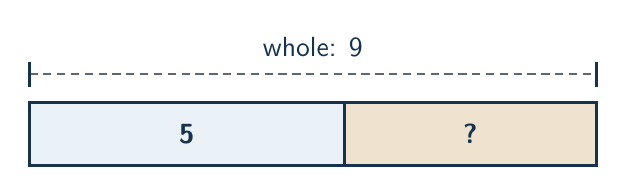
\begin{tikzpicture}[x=0.8cm,y=0.8cm]
  \draw[qra axis, fill=qraPale] (0,0) rectangle (5,1);
  \draw[qra axis, fill=qraGold!22] (5,0) rectangle (9,1);
  \node[qra label] at (2.5,0.5) {5};
  \node[qra label] at (7,0.5) {?};
  \draw[qra guide] (0,1.45) -- (9,1.45);
  \draw[qra tick] (0,1.25) -- (0,1.65);
  \draw[qra tick] (9,1.25) -- (9,1.65);
  \node[qra small label, above=3pt] at (4.5,1.45) {whole: 9};
\end{tikzpicture}
\end{document}
